\subsection{Неопределенный интеграл.}

 Дано: $f: \langle a,b\rangle \rightarrow \mathbb{R}$. $F$ называется \deff{первообразной} функция f, если:

\begin{enumerate}
    \item $F$ дифференцируема на $\langle a,b\rangle$.

    \item $\forall x \in \langle a,b\rangle: F'(x) = f(x) $.
\end{enumerate}

\thmm{Теорема 1}

$f$ - непрерывна на $\langle a,b \rangle$. Тогда $f$ имеет первообразную на $\langle a,b\rangle$.

\textbf{Доказательство:}
\begin{quote}
    <см теорема Барроу>
    
    \hfill Q.E.D.
\end{quote}

\thmm{Теорема 2}

$F$ - первообразная $f$ на $\langle a,b \rangle$. Тогда:
\begin{enumerate}
    \item $\forall c \in \mathbb{R}$: $F + c$ тоже первообразная.
    \item Если $G$ - еще одна первообразная f, то $F - G = const$.
\end{enumerate}
\textbf{Доказательство:}

    \begin{enumerate}
        \item воспользуемся арифметическим свойством производной. Тривиально.
        \item $(F-G)' = F' -G' =f-f= 0$. Пользуясь теоремами, так как производная везде $\geq 0$, то $F-G$ неубывающая. Аналогично так как производная на промежутке $\leq 0 $, то $F-G$ невозврастающая. Откуда это константа.
    \end{enumerate}
    \hfill Q.E.D.

\deff{Неопределенный интеграл} $f$ --- это множество всех первообразных $f$.

\textbf{Замечание от Славы.} Кохась подразумевает, что неопределенный интеграл это множество всех первообразных на том же интервале $\langle a,b \rangle$.

Обозначается неопределенный интеграл так:
$$\int f \quad \text{или} \int f(x) dx $$

Формально: $\displaystyle \int f(x)dx = F(x) +C$

\deff{Таблица неопределенных интегралов:}

Она переписывается из таблицы производных, просто в обратную сторону. Но есть две \uline{\emph{загадочные}} формулы:
     $$\displaystyle \int \cfrac{dx}{1-x^2} = \frac{1}{2}\ln \left|\cfrac{1+x}{1-x}\right| + C \quad \quad \int \cfrac{dx}{\sqrt{1+x^2}} = \ln \left|x + \sqrt{1+x^2}\right| + C$$

\thmm{Теорема (о св-вах неопределенного интервала)}

Пусть $f,g$ - имеют первообразную $F,G$ на $\langle a,b \rangle$. Тогда:

\begin{enumerate}
    \item $\dint (f+g) = \dint f + \dint g$
    \item $\forall a \in \mathbb{R}: \dint (af)=a\dint f$
    \item $\dint f(\varphi(t))\varphi'(t)dt = \left(\dint f(x)dx\right)\Big |_{x=\varphi(t)}= F(\varphi(t)) + C$
    \item частный случай. $\forall \alpha,\beta \in \mathbb{R}:\dint f(\alpha x + \beta) = \frac{1}{\alpha}F(\alpha x+\beta) + C$
    \item $f,g$ - дифф. на $\langle a,b\rangle$. Пусть $f'g$ и $fg'$ имеют первообразную: 
    
    Тогда: $\dint f g' = fg -\dint f'g$
\end{enumerate}

\textbf{Доказательство:}
\begin{enumerate}
    \item очевидно из свойств производной и теоремы 2.
    \item очевидно из свойств производной и теоремы 2.
    \item очевидно из производной композиции.
    \item очевидно из свойств производной и теоремы 2.
    \item Перенесите интеграл в правой части налево. Очевидно из произведения производных.
\end{enumerate}
    \hfill Q.E.D.

\textbf{Замечание.} Формула 3 часто будет использоваться для замены переменных в интегралах.
$$F(\varphi(t)) = \dint f(\varphi(t))\varphi'(t)dt $$
Давайте считать, что $\varphi $ обратима. Тогда $t = \varphi^{-1}(x)$. Подставим:
$$F(x)=\left(\dint f(\varphi(t))\varphi'(t)dt\right)\Big|_{t: = \varphi^{-1}(x)} $$

Для чего это? Благодаря этому, мы умеем вычислять первообразные немного по-другому. Мы можем подставлять вместо $x$ что-либо, а потом возвращаться обратно к $x$.

\subsection{Выпуклые функции.}

Множество $A \in R^m$ \deff{выпукло}, если:
$$\forall x,y \in A , [x,y]\subset A: [x,y] = \{x+t(y-x), t\in[0,1]\}$$
 $f:\langle a,b\rangle\rightarrow \mathbb{R}$ --- \deff{выпукла} на промежутке $\langle a,b\rangle$, если:
$$\forall x_1,x_2 \in \langle a,b \rangle: \forall \alpha \in[0,1]:f(\alpha x_1+(1-\alpha)x_2)\leq \alpha f(x_1) + (1-\alpha) f(x_2)$$

\deff{Надграфик} (f,$\langle c,d \rangle) = \{(x,y): x\in \langle c,d \rangle, y \geq f(x)  \}$

\textbf{Замечанние.} $f$ - выпукло на $\langle a,b\rangle \Leftrightarrow$ Надграфик $(f, \langle a,b \rangle)$ - выпуклый в $R^2$.

\thmm{Лемма (о трех хордах)}

$f$ - выпукла на $\langle a,b\rangle \Leftrightarrow \forall x_1<x_2<x_3 \in\langle a,b \rangle$ выполнено:
$$\cfrac{f(x_2)-f(x_1)}{x_2-x_1} \leq \cfrac{f(x_3)-f(x_1)}{x_3-x_1}\leq \cfrac{f(x_3)-f(x_2)}{x_3-x_2}$$
\textbf{Доказательство:}

Возьму первое неравенство. Домножу на знаменатели и оставлю плюсы:
$$(x_3-x_1) (f(x_2)-f(x_1)) \leq (x_2-x_1) (f(x_3)-f(x_1)$$
$$f(x_2)\leq \cfrac{x_2-x_1}{x_3-x_1}f(x_3) + \cfrac{x_3-x_2}{x_3-x_2}f(x_1)$$
Чего-то не хватает, вспомним, что $f(x_2) = f\left (\cfrac{x_2-x_1}{x_3-x_1}x_3 +\cfrac{x_3-x_2}{x_3-x_1}x_1\right)$. Ой, это же условие выпуклости. Так как все переходы равносильны, то 
это неравенство выполнено, когда $f$ выпукла. Второе неравенство решается аналогично (позже будет добавлено в конспект).
\hfill Q.E.D.

$f$ - \deff{строго выпукло} на $\langle a,b\rangle$:
$$\forall x_1,x_2 \in \langle a,b \rangle: \forall \alpha \in[0,1]:f(\alpha x_1+(1-\alpha)x_2)< \alpha f(x_1) + (1-\alpha) f(x_2)$$
Просто меняется знак на строгий.

\thmm{Теорема (об одностор. дифф-ти вып. функции)}

$f$ - выпукла на $\langle a,b \rangle$. Тогда $\forall x\in\langle a,b\rangle: \exists f'_+(x), f'_-(x)$,  а также

$\forall x_1<x_2\in \langle a,b\rangle$ выполнено:
$$f'_-(x_1)\leq f'_+(x_1) \leq \cfrac{f(x_2)-f(x_1)}{x_2-x_1}\leq f'_-(x_2)$$
\textbf{Доказательство:}

Сначала докажу, что $f'_-(x_1)\leq f'_+(x_1)$. Замечу, что $x_1$ в таком случае не должно быть граничной (иначе предела существовать просто не будет). Значит есть какая-то $s$ левее $x_1$ и какое-то $t$ правее $x_1$. Посмотрю на данные выражения:
$\cfrac{f(t)-f(x_1)}{t-x_1}$ и $\cfrac{f(c)-f(x_1)}{c-x_1}$. 

По теореме о трех хордах: $\cfrac{f(c)-f(x_1)}{c-x_1} \leq \cfrac{f(t)-f(x_1)}{t-x_1}$.

Замечу, что при устремлении $s$ к $x_1$,  $\cfrac{f(c)-f(x_1)}{c-x_1}$ будет увеличиваться по теореме о трех хордах (см изобр, напишите т. о трех хордах для $s,s',x_1$).

Замечу, что при устремлении $t$ к $x_1$,  $\cfrac{f(t)-f(x_1)}{t-x_1}$ будет  уменьшаться по теореме о трех хордах (см изобр, напишите т. о трех хордах для $x_1,t',t$).


\begin{center}
 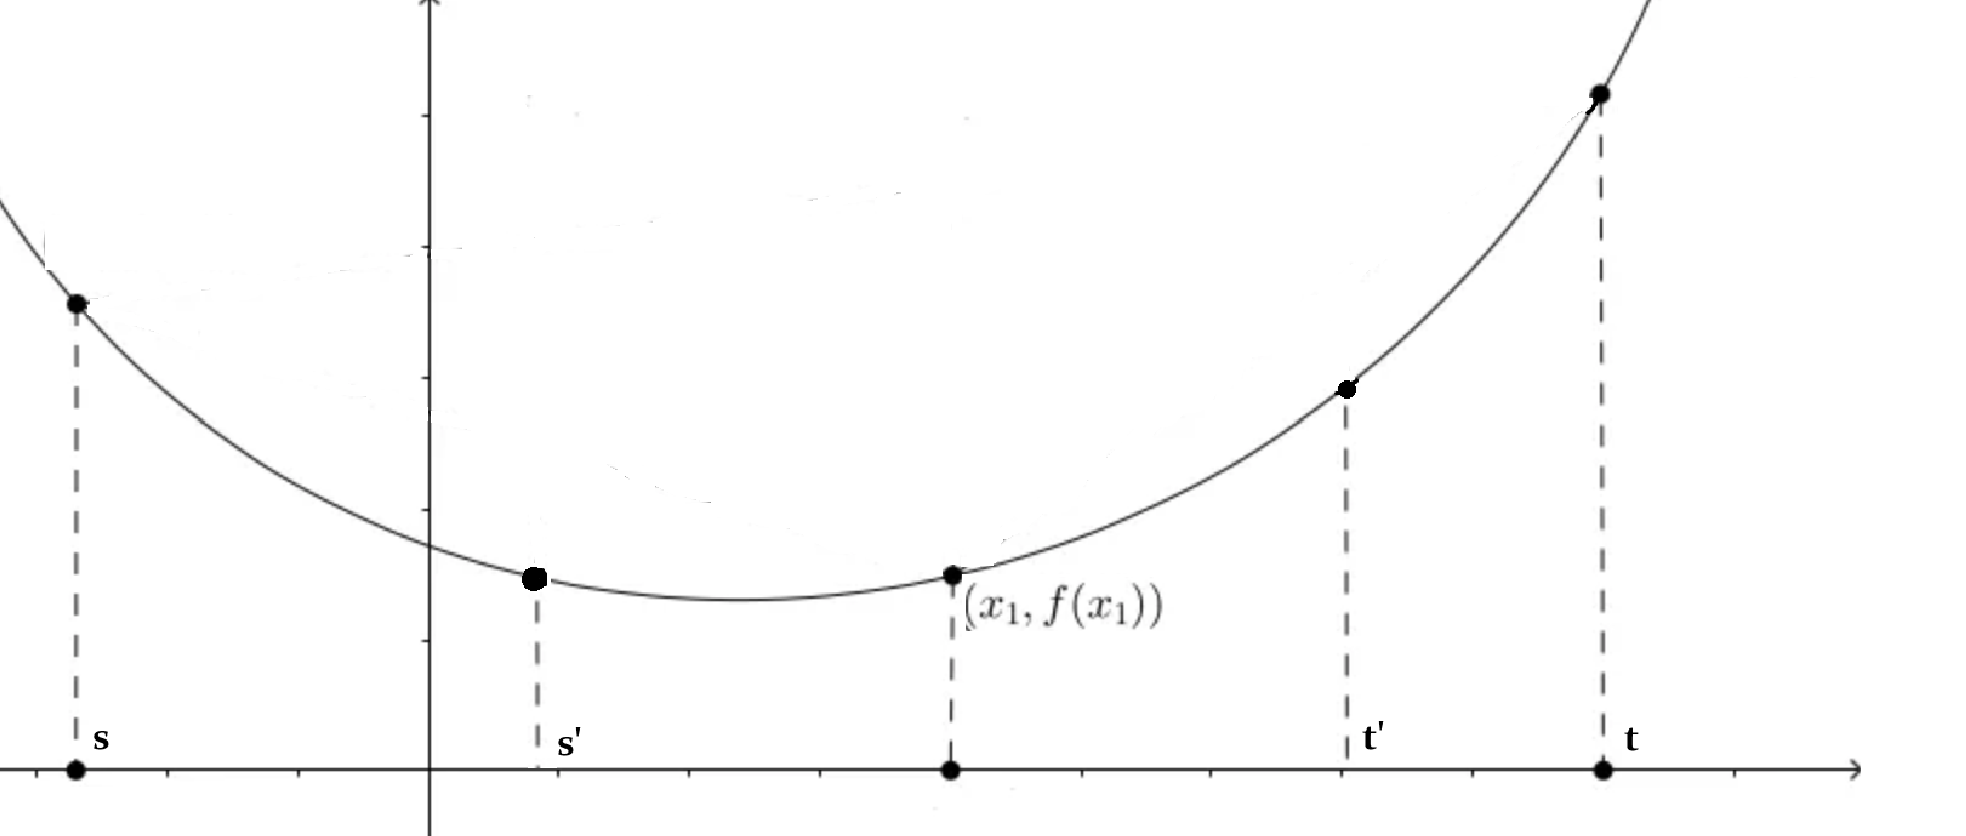
\includegraphics[width = 15cm]{assets/integral_1.png}
\end{center}

Заметим, что первая функция ограниченна сверху второй, а вторая ограниченна снизу первой. Откуда существуют  $f'_-(x_1), f'_+(x_1)$. Теперь применим теорему о предельном переходе в неравенствах и получим, что $f'_-(x_1)\leq f'_+(x_1)$.

Теперь докажем вторую часть.\\
Возьму $t$ на отрезке $(x_1,x_2)$. Посмотрю, на  $\cfrac{f(t)-f(x_1)}{t-x_1}$ и $\cfrac{f(t)-f(x_2)}{t-x_2}$

Заметим, что исходя из этого, тк монотонна возрастает на промежограниченна снизу и сверху (по тем же соображением, что и до этого)
$$\exists  \lim\limits_{t \rightarrow x_1 + 0}\cfrac{f(t)-f(x_1)}{t-x_1} = f'_+(x_1)$$ и тк $\cfrac{f(t)-f(x_1)}{t-x_1}\leq\cfrac{f(x_2)-f(x_1)}{x_2-x_1}$ по лемме о трех хордах, то выполнено второе неравенство.
$$\exists  \lim\limits_{t \rightarrow x_2 - 0}\cfrac{f(t)-f(x_2)}{t-x_2} = f'_-(x_2)$$ и тк $ \cfrac{f(x_2)-f(x_1)}{x_2-x_1}\leq \cfrac{f(t)-f(x_2)}{t-x_2}$ по лемме о трех хордах, то выполнено третье неравенство.

\hfill Q.E.D.

\subsection{Определенный интеграл.}


\deff{def:} \deff{Фигура} - это ограниченное подмножество в $R^2$. $\varepsilon$ - множество всех возможных фигур.

$\sigma: \varepsilon \rightarrow [0,+\infty)$ ---  назовем \deff{площадью}, если:
\begin{enumerate}
    \item Аддитивно: $A_1,A_2 \in \varepsilon, A_1\cap A_2 = \emptyset, \sigma(A_1\cup A_2) = \sigma(A_1)+\sigma(A_2)$
\item Нормировка: $\sigma ([a,b]\times[c,d]) = (b-a)(d-c)$.
\end{enumerate}

\textbf{Замечание.} Площади существуют.

\textbf{Замечание.} \begin{enumerate}
    \item Она обладает монотонностью по включению: $A \subset B, \sigma(A) \leq \sigma(B)$.
    \item $\sigma(\text{вертик отрезок})=0$.
\end{enumerate}

\deff{def:}  $\sigma:\varepsilon\rightarrow [0,+\infty)$---\deff{ослабленная площадь}, если выполнено:
\begin{enumerate}
    \item монотонна.
    \item нормированна.
    \item ослабленная адиттивность: Есть $E \in \varepsilon: l $ - вертик. прямая $L^-$ - левая полуплоскость, $L^{+1}$ - правая полуплоскость(замкнутая полуплоскость), тогда  $E_1 = E\cap L^-, E_2 = E \cap L^+: \sigma(E)=\sigma(E_1)+\sigma(E_2)$
\end{enumerate}

Пример осл. площади:
\begin{enumerate}
    \item $\sigma A = \inf (\sum \sigma(P_k), \text{где $A = \bigcup\limits_{\text{конеч}}P^k, \text{где $P_k$ - прямоугольник}$})$ 
    \item $\sigma A = \inf (\sum \sigma(P_k), \text{где} A = \bigcup P^k, \text{где $P_k$ - прямоугольник})$
\end{enumerate}

todo: написать отличие.

\deff{def:} \deff{Срезка} - $f:\langle a,b\rangle \rightarrow \mathbb{R} $.
\begin{enumerate}
    \item \uline{положительная} --- $f^+ = max(f,0)$
    \item \uline{отрицательная} --- $f^- = max(-f,0)$
\end{enumerate}

todo: вставить рисунок

\deff{def:} $f:[a,b] \rightarrow \mathbb{R}, f\geq 0$ ПГ $(f,[a,b]) = \{(x,y): x\in [a,b], y \in [0,f(x)]\}$.

\deff{def:} $f: [a,b] \rightarrow \mathbb{R}$, $f$ - непр., $\sigma $- осл. адд площадь, тогда определенный интегралом $f$ по отрезку $[a,b]$ назовем: $$\dint\limits_{a}^b f =\dint\limits_{a}^b f(x) dx =\sigma(\text{ПГ($f^+$,$[a,b]$)})-\sigma(\text{ПГ($f^-$,$[a,b]$)})$$

todo: тут что-то пропущено

\textbf{Свойство интеграла.}
\begin{enumerate}
    \item Аддитивность по промежутку: $\forall c \in [a,b]:\dint\limits_{a}^b =\dint\limits_{a}^c + \dint\limits_{c}^b $
    \item Монотонность: $f\leq g$ - непр., то $\dint\limits_{a}^b f(x)\leq \dint\limits_{a}^b g(x)$. 

    Говорят: Проинтегрируем неравенство $f\leq g$, на отрезке $[a,b]$.

    \item $(b-a)\min_{[a,b]} f \leq\integral{a}{b}f\leq (b-a)\max_{[a,b]}f$

    Делается с помощью монотонности и интегрирования $\min_{[a,b]}f\leq f\leq\max_{[a,b]}$

    \item $\left|\integral{a}{b}f(x)dx\right|\leq \integral{a}{b}|f(x)|dx$

    Проинтегрируем $-|f|\leq f\leq |f|$ и получим то, что хотим.

    \item \thmm{Теорема о среднем}

    Функция $f \in C([a,b])$. Тогда $\exists c \in [ab]$, тогда:
    $$\integral{a}{b}f = f(c)(b-a)$$
    \textbf{Доказательство:} 
    
    $a=b$ - скучно. Если $a\neq b$, напишем неравентсво п.3:
    $$\min f\leq \cfrac{1}{b-a}\integral{a}{b}f\leq \max f$$ А мы знаем, что функция непрерывна, поэтому $\exists c: c = \cfrac{1}{b-a}\integral{a}{b}f$. 
    
    \hfill Q.E.D.
\end{enumerate}

\deff{Интеграл с переменным верхним пределом} -  $\Phi:[a,b] \rightarrow R: \Phi(x)= \integral{a}{x}f$

\deff{Интеграл с переменным нижним пределом} -  $\psi:[a,b] \rightarrow R: \psi(x)= \integral{x}{b}f$

для $f\in C([a,b])$.

\thmm{Теорема (Барроу)}

В усл.определений. Доказать, что $\Phi$ дифф на $[a,b]$, $\Phi'(x)=f(x)$.

\textbf{Доказательство.}

$y> x: \lim\limits_{y \rightarrow x+0} \cfrac{\Phi(y)-\Phi(y)}{y-x} =\lim\limits_{y \rightarrow x+0} \cfrac{1}{y-x} \integral{x}{y}f =\lim_{y\rightarrow x+0} f(c), \text{где $c$ между $x,y$ из теоремы о среднем}$

Получим, что правосторонняя производна равна $f(x)$. Аналогично про левостороннюю. Откуда производная это $f(x)$.

 \hfill Q.E.D.
 
\textbf{Замечание} Мы построили первообразную для функции $f$.

\thmm{Теорема (формула Ньютона-Лейбница)}

$f\in C([a,b])$, $F$ - первообразная $f$ на $[a,b]$. Тогда

$\integral{a}{b}f(x)dx = F(b)-F(a) = F(x)\big|^b_a$

\textbf{Доказательство:}

$F = \Phi + c$, по теореме 2. Поэтому сделаем некоторые преобразования:
$$\integral{a}{b}f(x)dx = \Phi(b)= \Phi(b)-\Phi(a) = (F(b)-c)-(F(a)-c)=F(b)-F(a)$$
 \hfill Q.E.D.

 \textbf{Следствие:} Этот определенный интеграл независит от выбора $\sigma$. 
 
 \textbf{Замечание:} Откажемся от соглашения $a\leq b$ и введем для $d<c:$
 $$\integral{c}{d}= - \integral{d}{c} = F(d) - F(c)$$
 \thmm{Микротеорема (Линейность интеграла)}

 Для $f,g \in C([a,b])$, $\alpha,\beta \in \mathbb{R}$, выполнено:
$$\integral{a}{b}\alpha f+ \beta g = \alpha \integral{a}{b}f + \beta\integral{a}{b}g$$
\textbf{Доказательство:}

$(\alpha F+\beta G)\big|^b_a = \alpha F\big|^b_a + \beta F|^b_a$ из линейности неопредел. интеграла.
 \hfill Q.E.D.

 \thmm{Теорема (Интегрирование по частям)}

 $f',g \in C([a,b])$. Тогда $\integral{a}{b}fg' = fg\big|_a^b-\integral{a}{b}f'g$

 \textbf{Доказательство}

Из теоремы  о свойствах неопределенного интеграла:
$$fg = \text{првобр} (fg'+f'g) \Rightarrow \integral{a}{b}(fg' + f'g) = fg\big|_{a}^b$$
 \hfill Q.E.D.
 
 \thmm{Теорема (о замене переменных)}

$f \in C(\langle a,b\rangle), \varphi\langle\alpha, \beta\rangle \rightarrow \varphi \in C^1, [p,q] \in \langle \alpha,\beta\rangle$. Тогда:

$$\integral{p}{q}f(\varphi(t))\varphi'(t)dt = \integral{\varphi(p)}{\varphi(q)}f(x)dx$$

\textbf{Доказательство}

$F$ - первообразная $f$, тогда $F(\varphi(t))$ - первообразная $f(\varphi(t))\varphi'(t)$ и все получается.
 
 \hfill Q.E.D.

1:09 мат анализ кохась лекция 2. Я ничего не понял про нижние два замечания


 \textbf{Замечание.} Может показаться, что множество $\varphi([p,q])$ шире $[\varphi(p),\varphi(q)]$. 

 \textbf{Замечание.} Может быть, что $\varphi(p) > \varphi(q)$

 \thmm{Неравен}